\documentclass[12pt]{article}
\usepackage{graphicx}
\usepackage[czech]{babel}
\usepackage[utf8]{inputenc}
\usepackage{titling}
\usepackage{pdfpages}
\usepackage[nopar]{lipsum}
\usepackage{mathtools}
\usepackage{multirow}
\usepackage{caption}
\usepackage{float}
\usepackage{enumitem}
\usepackage{listings}
\usepackage{amsmath}
\usepackage{amssymb}
\usepackage{amsmath}
\newcommand*{\escape}[1]{\texttt{\textbackslash#1}}


\setlength{\hoffset}{-1cm}
\setlength{\voffset}{-2cm}
\setlength{\textwidth}{15cm}
\setlength{\textheight}{23cm}


\begin{document}
	
	\title{Semestrální práce}
\author{Filip Polák}
\date{Akademický rok 2020/2021}
\begin{titlepage}
	\begin{center}
		
\includegraphics[scale=0.6]{logo_zcu}\\
		\vspace{2cm}
		\begin{large}
			\textbf{\thetitle}\\
		\end{large}
		
		\vspace{3cm}
		\theauthor\\
		\vspace{5cm}
		\thedate
	\end{center}
\end{titlepage}

	\newpage
	\section{Mycroft}
	Mycroft je open source hlasový asistent vytvořený společností Mycroft AI, který je možné spustit na počítači či notebooku s operačním systémem Linux, v autě nebo na mobilu s operačním systémem Android. Hlavním tahákem jsou ale Mark I a Mark II, které představují alternativu k Google Home či Amazon Echo a slouží k ovládání domácnosti. Ve svých počátcích byl projekt podpořen kampaní na Kickstarteru, kde na něj uživatelé přispěli přes 120 000\textdollar. Jedním z hlavních důvodů úspěchů této kampaně byly skandály velkých hráčů v oboru hlasových asistentů se sdílením dat uživatelů třetím stranám, které otevřely cestu menším společnostem, které si zakládají na ochraně uživatelských dat a uživatelích jako takových.

	\begin{figure}[H] 
		\begin{center}
			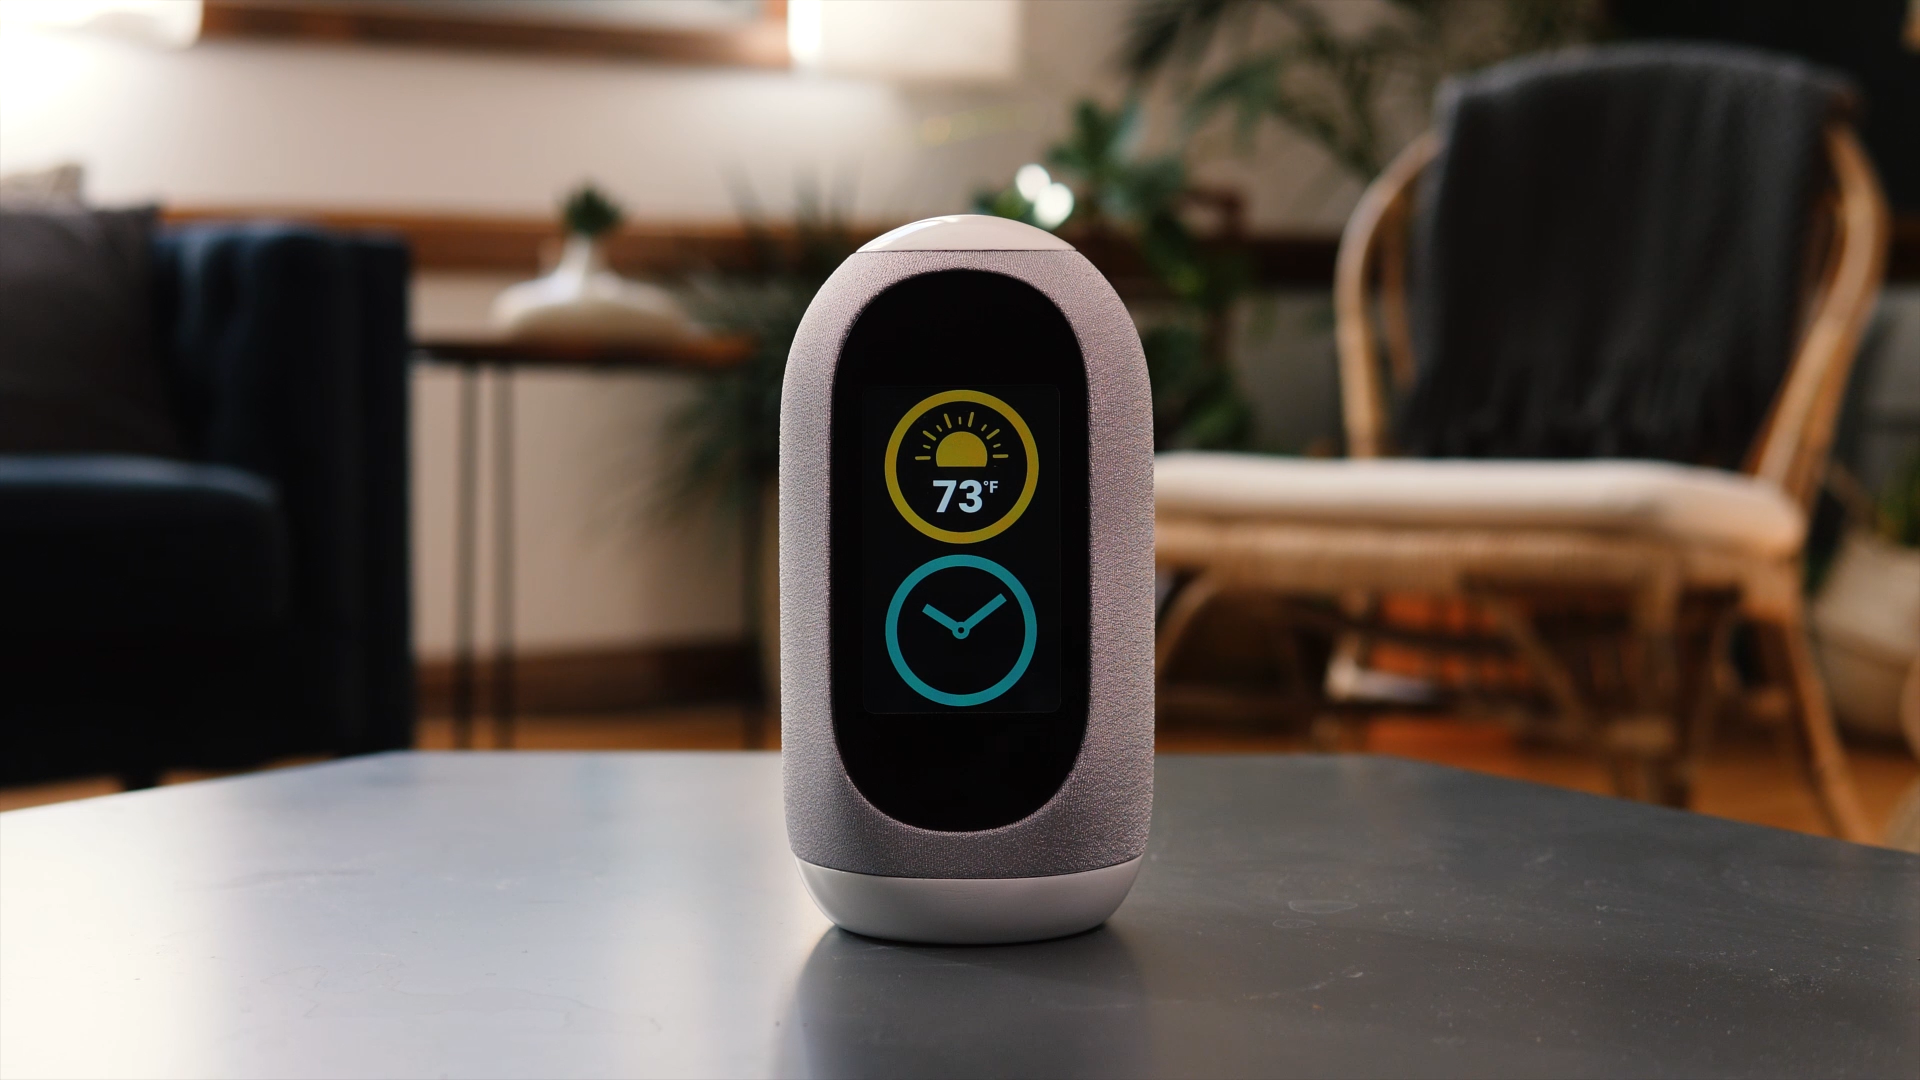
\includegraphics[scale=.20]{figures/mark_II}
			\caption{Mark II}\label{fig:mark_II}
		\end{center}
	\end{figure}
	\subsection{Skills}
	Každý hlasový dialogový systém musí mít definovanou doménu, ve které se bude konverzace provádět. Tato definice je v Mycroftu elegantně provedena pomocí tzv. Skills (dovedností). Skills jsou vytvářeny techniky a programátory přímo v Mycroftu AI, ale možnost přispět k rozšíření novými či zlepšení již existujících Skills mají i samotný uživatelé.

	
	\end{document}